\documentclass{beamer}
\usetheme{CambridgeUS}
\usepackage[utf8]{vietnam}
\usepackage{hyperref}
\usepackage{graphicx}
\usepackage{caption}
\usepackage{enumerate}
\usepackage{multicol}
%%\usepackage{enumitem}
\usepackage{subcaption}
\graphicspath{ {Img/} }

%%--------------------------------------------------------

\title{Mutilobjective Evolutionary Optimization}
\author{TaskOverflow}




%%--------------------------------------------------------

\begin{document}
    \maketitle 

%%---------------------------------------------------------

    \section{INTRODUCTION}
    \begin{frame}{INTRODUTION}
        \begin{block}{Point 1}
            Thế nào là bài toán tối ưu đa mục tiêu?
        \end{block}
    \end{frame}
    
    \begin{frame}{Các định nghĩa cơ bản}
        \begin{block}{Không gian nghiệm}
            Với các điều kiện rằng buộc của $x$ sẽ xác định một không gian $\Omega \subset R^{n}$
        \end{block}
        \pause
        \begin{block}{Hàm mục tiêu}
                $y = f(x)= (f_{1}(x),...,f_{m}(x))$
                \\$ x \in \Omega $
        \end{block}
        \pause
        \begin{block}{Không gian mục tiêu}
            $f : \Omega \to \Theta  \subset R^{m}$ xác định không gian mục tiêu $\Theta$
        \end{block}
    \end{frame}

    \begin{frame}{Hình ảnh minh họa}
        \begin{figure}
        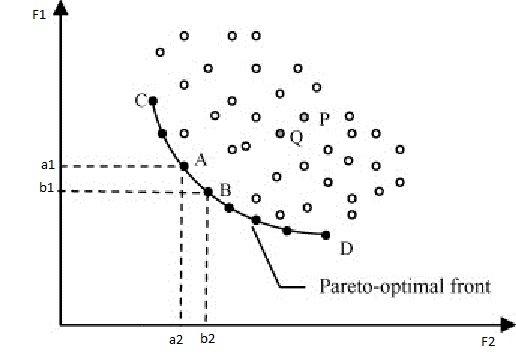
\includegraphics[scale = 0.6]{paretofront.jpg}
        \caption{Nguồn: Semantic Scholar}
        \end{figure}
    \end{frame}
    \begin{frame}{Các định nghĩa cơ bản}
        \begin{columns}
        \column{0.6\textwidth}
        \begin{figure}
            \centering
            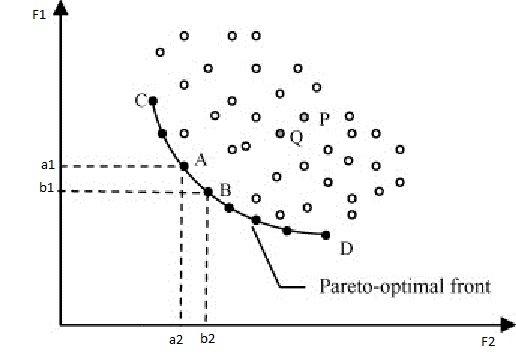
\includegraphics[scale = 0.5]{paretofront.jpg}
            \caption{Hình ảnh minh họa}
            \label{fig:my_label}
        \end{figure}
        \column{0.4\textwidth}
        \pause
        Cho 2 nghiệm $x,y \in \Omega $, $x$ trội hơn $y$ nếu như $\forall i \in {1,2,...,m}, f_{i}(x) \leq f_{i}(y)$ và $ \exists j \in {1,2,...,m}, f_{j}(x) < f_{j}(y)$. 
        \end{columns}
    \end{frame}
    \begin{frame}{Các định nghĩa cơ bản}
        \begin{columns}
        \column{0.6\textwidth}
        \begin{figure}
            \centering
            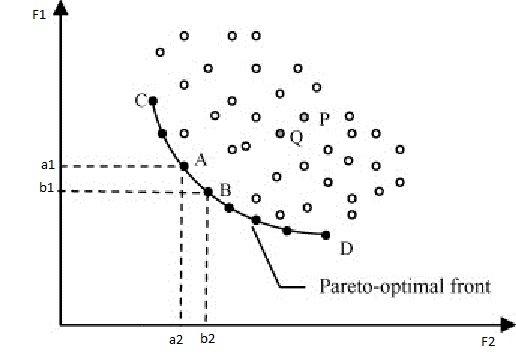
\includegraphics[scale = 0.5]{paretofront.jpg}
            \caption{Hình ảnh minh họa}
            \label{fig:my_label}
        \end{figure}
        \column{0.4\textwidth}
        Một nghiệm $x^{*} \in \Omega$ là nghiệm tối ưu Pareto nếu không tồn tại $x \in \Omega$ trội hơn nó.
        \end{columns}
    \end{frame}
    \begin{frame}{Các định nghĩa cơ bản}
        \begin{columns}
        \column{0.6\textwidth}
        \begin{figure}
            \centering
            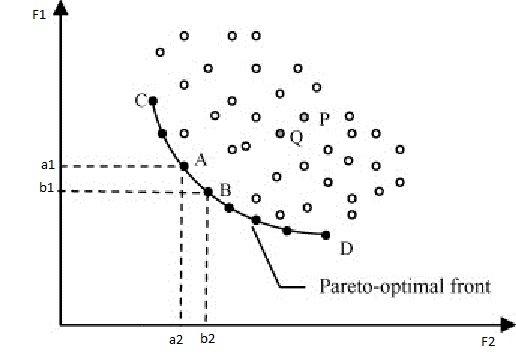
\includegraphics[scale = 0.5]{paretofront.jpg}
            \caption{Hình ảnh minh họa}
            \label{fig:my_label}
        \end{figure}
        \column{0.4\textwidth}
        Tập hợp nghiệm tối ưu Pareto được gọi là tập Pareto.
        \end{columns}
    \end{frame}
    \begin{frame}{Các định nghĩa cơ bản}
        \begin{columns}
        \column{0.6\textwidth}
        \begin{figure}
            \centering
            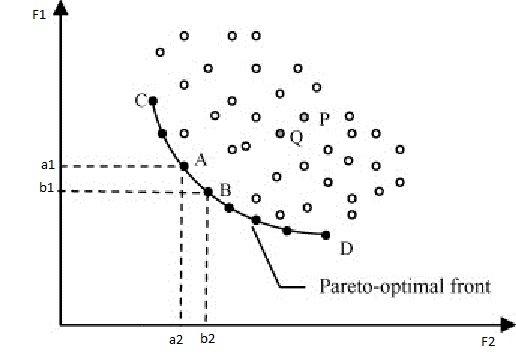
\includegraphics[scale = 0.5]{paretofront.jpg}
            \caption{Hình ảnh minh họa}
            \label{fig:my_label}
        \end{figure}
        \column{0.4\textwidth}
        Các vector mục tiêu tương ứng của tập Pareto được gọi là Biên Pareto (Pareto Frontier - PF).
        \end{columns}
    \end{frame}
    \begin{frame}{Mục tiêu tối ưu}
        Mục tiêu tối ưu là đạt được một tập xấp xỉ S với tập biên Pareto thỏa mãn:
        \pause
        \begin{block}{Độ hội tụ}
            Mọi nghiệm thuộc S là gần nhất có thể với P.
            \end{block}
        \pause
        \begin{block}{Độ đa dạng}
        Mọi nghiệm thuộc S phân bố đa dạng trên không gian mục tiêu
        \end{block}
    \end{frame}
    \begin{frame}{Hình ảnh minh họa}
        \begin{figure}
        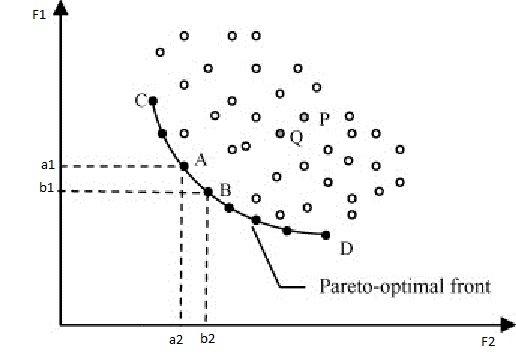
\includegraphics[scale = 0.6]{paretofront.jpg}
        \caption{Nguồn: Science Direct}
        \end{figure}
    \end{frame}

%%---------------------------------------------------------

\section{\textbf{Các thuật toán}}
\subsection{\textbf{Thuật toán NSGA-II}}

    \begin{frame}
    \frametitle{\textbf{Thuật toán NSGA-II}}
        \begin{itemize}
            \item<1-> Sau lần chạy thứ $ t $, duy trì một quần thể solution $ P_t $ có kích thước $ N $ cố định qua mọi lần chạy.
            \item<2-> Trong lần chạy thứ $ t + 1 $:
            \begin{enumerate}
                \item<2-> Sử dụng các toán tử selection, crossover và mutation để tạo ra quần thể con cháu $ Q_t $ từ $ P_t $.
                \item<2-> Chọn ra N phần tử tốt nhất từ $ P_t \cup Q_t $ để tạo ra $ P_{t + 1} $.
            \end{enumerate}
            \item<3-> Tính chất đặc trưng: Để đánh giá các solution trong bước (2), thuật toán sử dụng:
            \begin{enumerate}
                \item<3-> Sắp xếp bất thống trị (fast nondominated sorting) để chọn ra phần tử thống trị các phần tử khác.
                \item<3-> khoảng cách quần thể (crowding distance) để đảm bảo sự đa dạng của quần thể.
            \end{enumerate}
            \item<4-> Độ phức tạp: $ O(mN^2) $ mỗi lần chạy, với $ m $ là số mục tiêu.
        \end{itemize}
    \end{frame}

    \begin{frame}
    \frametitle{\textbf{Các đặc tính}}
        \begin{itemize}
            \item<1-> \textbf{Độ hội tụ:} NSGA-II sử dụng Fast nondominated sorting để sắp xếp lại các 
            cá thể trong $ P_t \cup Q_t $, sau đó ưu tiên giữ lại các cá thể ít bị thống trị nhất.
            \item<2-> \textbf{Độ đa dạng:} NSGA-II sử dụng Crowding distance để tính tổng khoảng 
            cách giữa các cá thể theo từng mục tiêu của bài toán, sau đó chọn ra các cá thể cách nhau 
            xa nhất. Như vậy các cá thể được chọn sẽ trải đều trên tập.
        \end{itemize}
    \end{frame}

%%---------------------------------------------------------    

\subsection{\textbf{Thuật toán MOEA/D}}

    \begin{frame}
    \frametitle{\textbf{Thuật toán MOEA/D}}
        \begin{itemize} 
            \item<1-> Khởi tạo một quần thể gồm $ N $ cá thể. Mỗi cá thể có vector $ \lambda_{i} $ được khởi tạo ngẫu nhiên và
                    mảng $ B(i) $ chứa $ T $ chỉ số cá thể hàng xóm có khoảng các Euclid theo $ \lambda $ gần với i nhất.
            \item<2-> Sau mỗi lần chạy duy trì một một tập quần thể $ EP $ (External Population) để lưu
                    lại các cá thể tốt nhất tính đến hiện tại.
        \end{itemize}
    \end{frame}

    \begin{frame}
    \frametitle{\textbf{Thuật toán MOEA/D}} 
        \begin{itemize}
            \item<1-> Trong lần chạy thứ $ t $:
            \item<2-> Duyệt $ \forall $ i:
            \begin{enumerate}
                \item<2-> Chọn 2 chỉ số ngẫu nhiên $ k $, $ l $ từ trong các hàng xóm của $ i $.
                \item<2-> Dùng các toán tử crossover, mutation để tạo ra cá thể con cháu/
                \item<2-> Nếu cá thể con cháu vi phạm ràng buộc thì dùng một thuật toán sửa chữa để tạo thành một
                cá thể con cháu mới thỏa mãn ràng buộc.
                \item<3-> So sánh cá thể con cháu với các hàng xóm của $ i $. 
                \item<3-> So sánh với các cá thể trong $ EP $.
            \end{enumerate}
            \item<4-> Độ phức tạp: $ O(mNT) $.
        \end{itemize}
    \end{frame}

    \begin{frame}
    \frametitle{\textbf{Các đặc tính}}
        \begin{itemize}
            \item<1-> \textbf{Độ hội tụ:} MOEA/D sử dụng một hàm hội tụ (Agression function)
            để so sánh giữa cá thể con cháu sinh ra và các hàm xóm của nó.
            \item<2-> \textbf{Độ đa dạng:} Bằng việc sinh ra con cháu từ việc chọn ngẫu
            nhiên từ đời cha là 2 hàng xóm, độ đa dạng của đời con cháu được đảm bảo.
        \end{itemize}
    \end{frame}

%%------------------------------------------------------------------    

    \begin{frame}
    \frametitle{\textbf{Thực nghiệm: Bài toán ZDT3}}
        \begin{itemize}
            \item Hàm mục tiêu:
            \begin{itemize}
                \item $ f_1(x) = x_1 $
                \item $ f_2(x) = g(x) \left[ 1 - \left( \dfrac{f_1(x)}{g(x)} \right)^2 \right] $, với
                $$ g(x) = 1 +\dfrac{9 \left( \sum\limits_{i = 2}^n x_i \right)}{(n - 1)} $$
            \end{itemize}
            \item Miền tìm kiếm: $ x = (x_1,..., x_n)^T \in \left[0, 1\right]^T $.
            \item Biên Pareto: Không liên tục, lồi.
        \end{itemize}
    \end{frame}

    \begin{frame} 
    \frametitle{\textbf{Thực nghiệm: Bài toán ZDT3}}
        \begin{figure}[!h]
            \center
            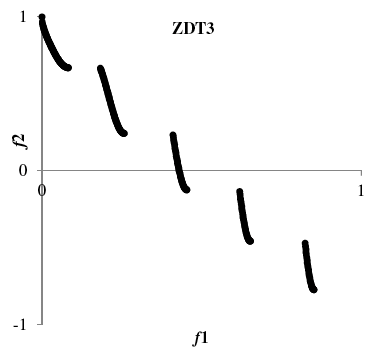
\includegraphics[width=0.5\linewidth]{zdt3-pf}
            \caption{Nguồn: Semantic Scholar}
        \end{figure}

    \end{frame}

%%-------------------------------------------------------
    
    \begin{frame}
    \frametitle{\textbf{So sánh giữa NSGA-II và MOEA/D}}
        \begin{itemize}
            \item Độ phức tạp mỗi lần chạy của MOEA/D nhỏ hơn NSGA-II. \pause
            \item NSGA-II chỉ cần một hệ số ngoài là mật độ đột biến (mutation rate) khi chạy thuật toán. \pause
            \item NSGA-II hội tụ tới biên Pareto nhanh hơn. \pause
            \item NSGA-II đảm bảo kích cỡ quần thể cố định $\implies$ dễ quản lý và lưu trữ hơn. \pause
        \end{itemize}
        \textbf{\href{https://youtu.be/ar0ZAMzuaz4}{Tại sao lại phải nghiên cứu và sử dụng MOEA/D?}}
    \end{frame}

%%---------------------------------------------------------

\section{Các bài toán nhiều mục tiêu}

    \begin{frame}{Many Objectives Problems (MoAPs)}
        \begin{itemize}
            \item <1-> Không có định nghĩa chung cho MaOPs.
            \item <2-> Động lực chính đằng sau MaOPs là làm nổi bật những thách thức đặt ra bởi một số lượng lớn các mục tiêu cho các thuật toán tiến hóa đa mục tiêu (MOEAs) hiện tại.
            \item <3-> Hiện tại ta có thể định nghĩa MaOPs là các bài toán đa mục tiêu MOPs với $m \geq 4$.
        \end{itemize}
    \end{frame}

    \begin{frame}{Khó khăn trong quá trình giải quyết MoAPs}
        \begin{itemize}
            \item <1-> Phần lớn các cá thể là không trội, không thể sắp xếp được.
            \item <2-> Tính toán độ đa dạng thuật toán trở nên khó khăn.
            \item <3-> Quá trình tái tổ hợp có thể không hiệu quả.
            \item <4-> Việc thể hiện trade-off surface khó khăn.
            \item <5-> Tốn thời gian để so sánh hiệu suất giữa các thuật toán với nhau (Performance metrics).
            \item <6-> Rất khó để biểu diễn lời giải một cách trực quan.
        \end{itemize}
    \end{frame}

    \begin{frame}{Hai ý tưởng cho các thuật toán Tiến hóa Tối ưu Nhiều mục tiêu - EMO}
        \begin{block}{1.}
            Sử dụng nguyên tắc trội đặc biệt: $ \epsilon $-Domination, các chiến lược hạn chế giao phối (Mating Restriction Scheme)
            hoặc chiến lược tái tổ hợp đặc biệt (Special Recombination Scheme như SBX với distribution index lớn, ...).
        \end{block}
        \pause
        \begin{block}{2.}
            Sử dụng nền tảng của các nghiên cứu đa mục tiêu trước.
        \end{block}
    \end{frame}
    
    \begin{frame}{Một số thuật toán tiến hóa để giải quyết các bài toái MoAPs hiện tại}
        \begin{multicols}{2}
        \begin{itemize}
            \item MSOPS-II
            \item MOEA/D
            \item HypE
            \item PICEA-g
            \item SDE
            \item GrEA
            \item NSGA-III
            \item KnEA
            \item RVEA
            \item Two-Arch 2
            \item $ \phi $ - DEA
            \item MOEA/DD
            \item AnD
        \end{itemize}
        \end{multicols}
    \end{frame}

\end{document}